\chapter{Introducción}
\label{cap:Introduccion}

Este capítulo aborda la motivación\index{motivación} del trabajo. Se trata de señalar la necesidad que lo origina, su actualidad y pertinencia. Puede incluir también un estado de la cuestión (o estado del arte) en la que se revisen estudios o desarrollos previos y en qué medida sirven de base al trabajo que se presenta.

En este capítulo debería introducirse el \emph{contexto disciplinar y tecnológico} en el que se desarrolla el trabajo de modo que pueda entenderse con facilidad el ámbito y alcance del TFG.\index{TFG} Puesto que un TFG no tiene que ser necesariamente un trabajo con aportes novedosos u originales, sólo es necesario la inclusión de <<estado del arte>> cuando este contribuya a aclarar aspectos clave del TFG o se desee justificar la originalidad del trabajo realizado.

A continuación se muestran algunos ejemplos para la inclusión de elementos en el documento como listas, tablas y figuras.

\noindent \textsc{IMPORTANTE}: \emph{A la hora de redactar el texto se debe poner especial atención en no cometer plagio\index{plagio} y respetar los derechos de propiedad intelectual \cite{refer00,sidney00}. En particular merece gran atención la inclusión de figuras e imágenes procedentes de Internet que no sean de elaboración propia. En este sentido se recomienda consultar el manual de la Universidad de Cantabria en el que se explica de modo conciso cómo incluir imágenes en un trabajo académico %\cite{unican18}
.}

% ------------------------------------------------------------------------------
% Ejemplos para la plantilla
% ------------------------------------------------------------------------------
\section{Ejemplos de listas}
\label{sec:ejListas}
\index{ejemplos} % Véase cómo se incluyen entradas en el índice alfabético
A continuación se van a añadir algunos ejemplos que pueden emplearse al redactar la memoria.

\index{ejemplos!listas} % Para el índice
\noindent Ejemplo de lista con \emph{bullet} especial.\index{lista!bullet} 
% Ejemplo: Lista con bullets especiales
% ============
\begin{itemize}
	\item[\ding{52}] peras
	\item manzanas
	\item naranjas
\end{itemize}


\noindent Ejemplo de lista en varias columnas.\index{lista!columnas}
% Ejemplo: Listas en varias columnas
% ============
\begin{multicols}{2} % El parámetro es el número de columnas de la lista
	\begin{enumerate}
		\item peras
		\item manzanas
		\item naranjas
		\item patatas
		\item calabazas
		\item fresas
	\end{enumerate}
\end{multicols}

\noindent Las listas se pueden personalizar (aunque debería estar justificado el cambiar el estilo por defecto, haciéndolo con mucha prudencia):

% Ejemplo:
% ============
\begin{dingautolist}{202} % Lista con símbolos sucesivos de la tabla dingbat
	\item peras
	\item manzanas
	\item naranjas
\end{dingautolist}


\section{Ejemplos de tablas}
\label{sec:ejTablas}
\index{ejemplos!tablas}
A continuación se incluyen algunos ejemplos de tablas\index{tabla} hechas con 
\LaTeX{} y paquetes dedicados.

% Ejemplo: Tabla con macro \cline
% ==========
\begin{table}[htb]%
	\centering
	\caption{Ejemplo de uso de la macro \texttt{cline}}
	\label{tab:cline}
	\begin{tabular}[t]{|r|l|}
		\hline
		7C0 & hexadecimal \\[1cm] % Ejemplo de separación fijada entre líneas
		3700 & octal \\ \cline{2-2}
		11111000000 & binario \\
		\hline \hline
		1984 & decimal \\
		\hline
	\end{tabular}
\end{table}


\noindent Ejemplo de tabla\index{tabla!ancho controlado} en la que se 
controla el ancho de la celda.

% Ejemplo: Ejemplo de tabla con control de la anchura de celda.
% ==========
\begin{table}[htb]%
	\centering
	\caption{Ejemplo de tabla con especificación de anchura de columna}
	\label{tab:anchura}
	\begin{tabular}{ | l | l | l | p{5cm} |}
		\hline
		Día & Temp Mín (\textdegree C) & Temp Máx (\textdegree C) & Previsión \\ \hline
		Lunes & 11 & 22 & Día claro y muy soleado. Sin embargo, la brisa de la tarde puede hacer que las temperaturas desciendan \\ \hline
		Martes & 9 & 19 & Nuboso con chubascos en muchas regiones. En Cataluña claro con posibilidad de bancos nubosos al norte de la región \\ \hline
		Miércoles & 10 & 21 & La lluvia continuará por la mañana pero las 
		condiciones climáticas mejorarán considerablemente por la tarde\\
		\hline
	\end{tabular}
\end{table}

\clearpage


\section{Ejemplos de figuras}
\label{sec:ejFiguras}
\index{ejemplos!figuras}

En esta sección se añaden ejemplos de muestra para la inclusión de 
figuras\index{figuras} simples y subfiguras.

% Ejemplo: Ejemplo de inclusión de figura
% ============
\begin{figure}[htb]
	\centering
	\includegraphics[width=0.8\linewidth]{clockCR}
	\caption[Ejemplo de figura]{Fotografía a color 
	(por J. Salido, CC BY-NC-ND)}
	\label{fig:ejFigure}
\end{figure}


\noindent Ejemplo de figuras compuestas por subfiguras incluidas con paquete \texttt{subcaption}.\index{figuras!subfiguras}\footnote{\url{https://osl.ugr.es/CTAN/macros/latex/contrib/caption/subcaption.pdftext}}


% Ejemplo: Ejemplo de inclusión de subfiguras
% ============
\begin{figure}[htb]
	\centering
	\begin{subfigure}[b]{0.4\linewidth}
		\centering
		\includegraphics[width=0.8\linewidth]{clockCR}
		\caption{Fotografía a color}\label{fig:fotocolor}
	\end{subfigure} 
	\begin{subfigure}[b]{0.4\linewidth}
		\centering
		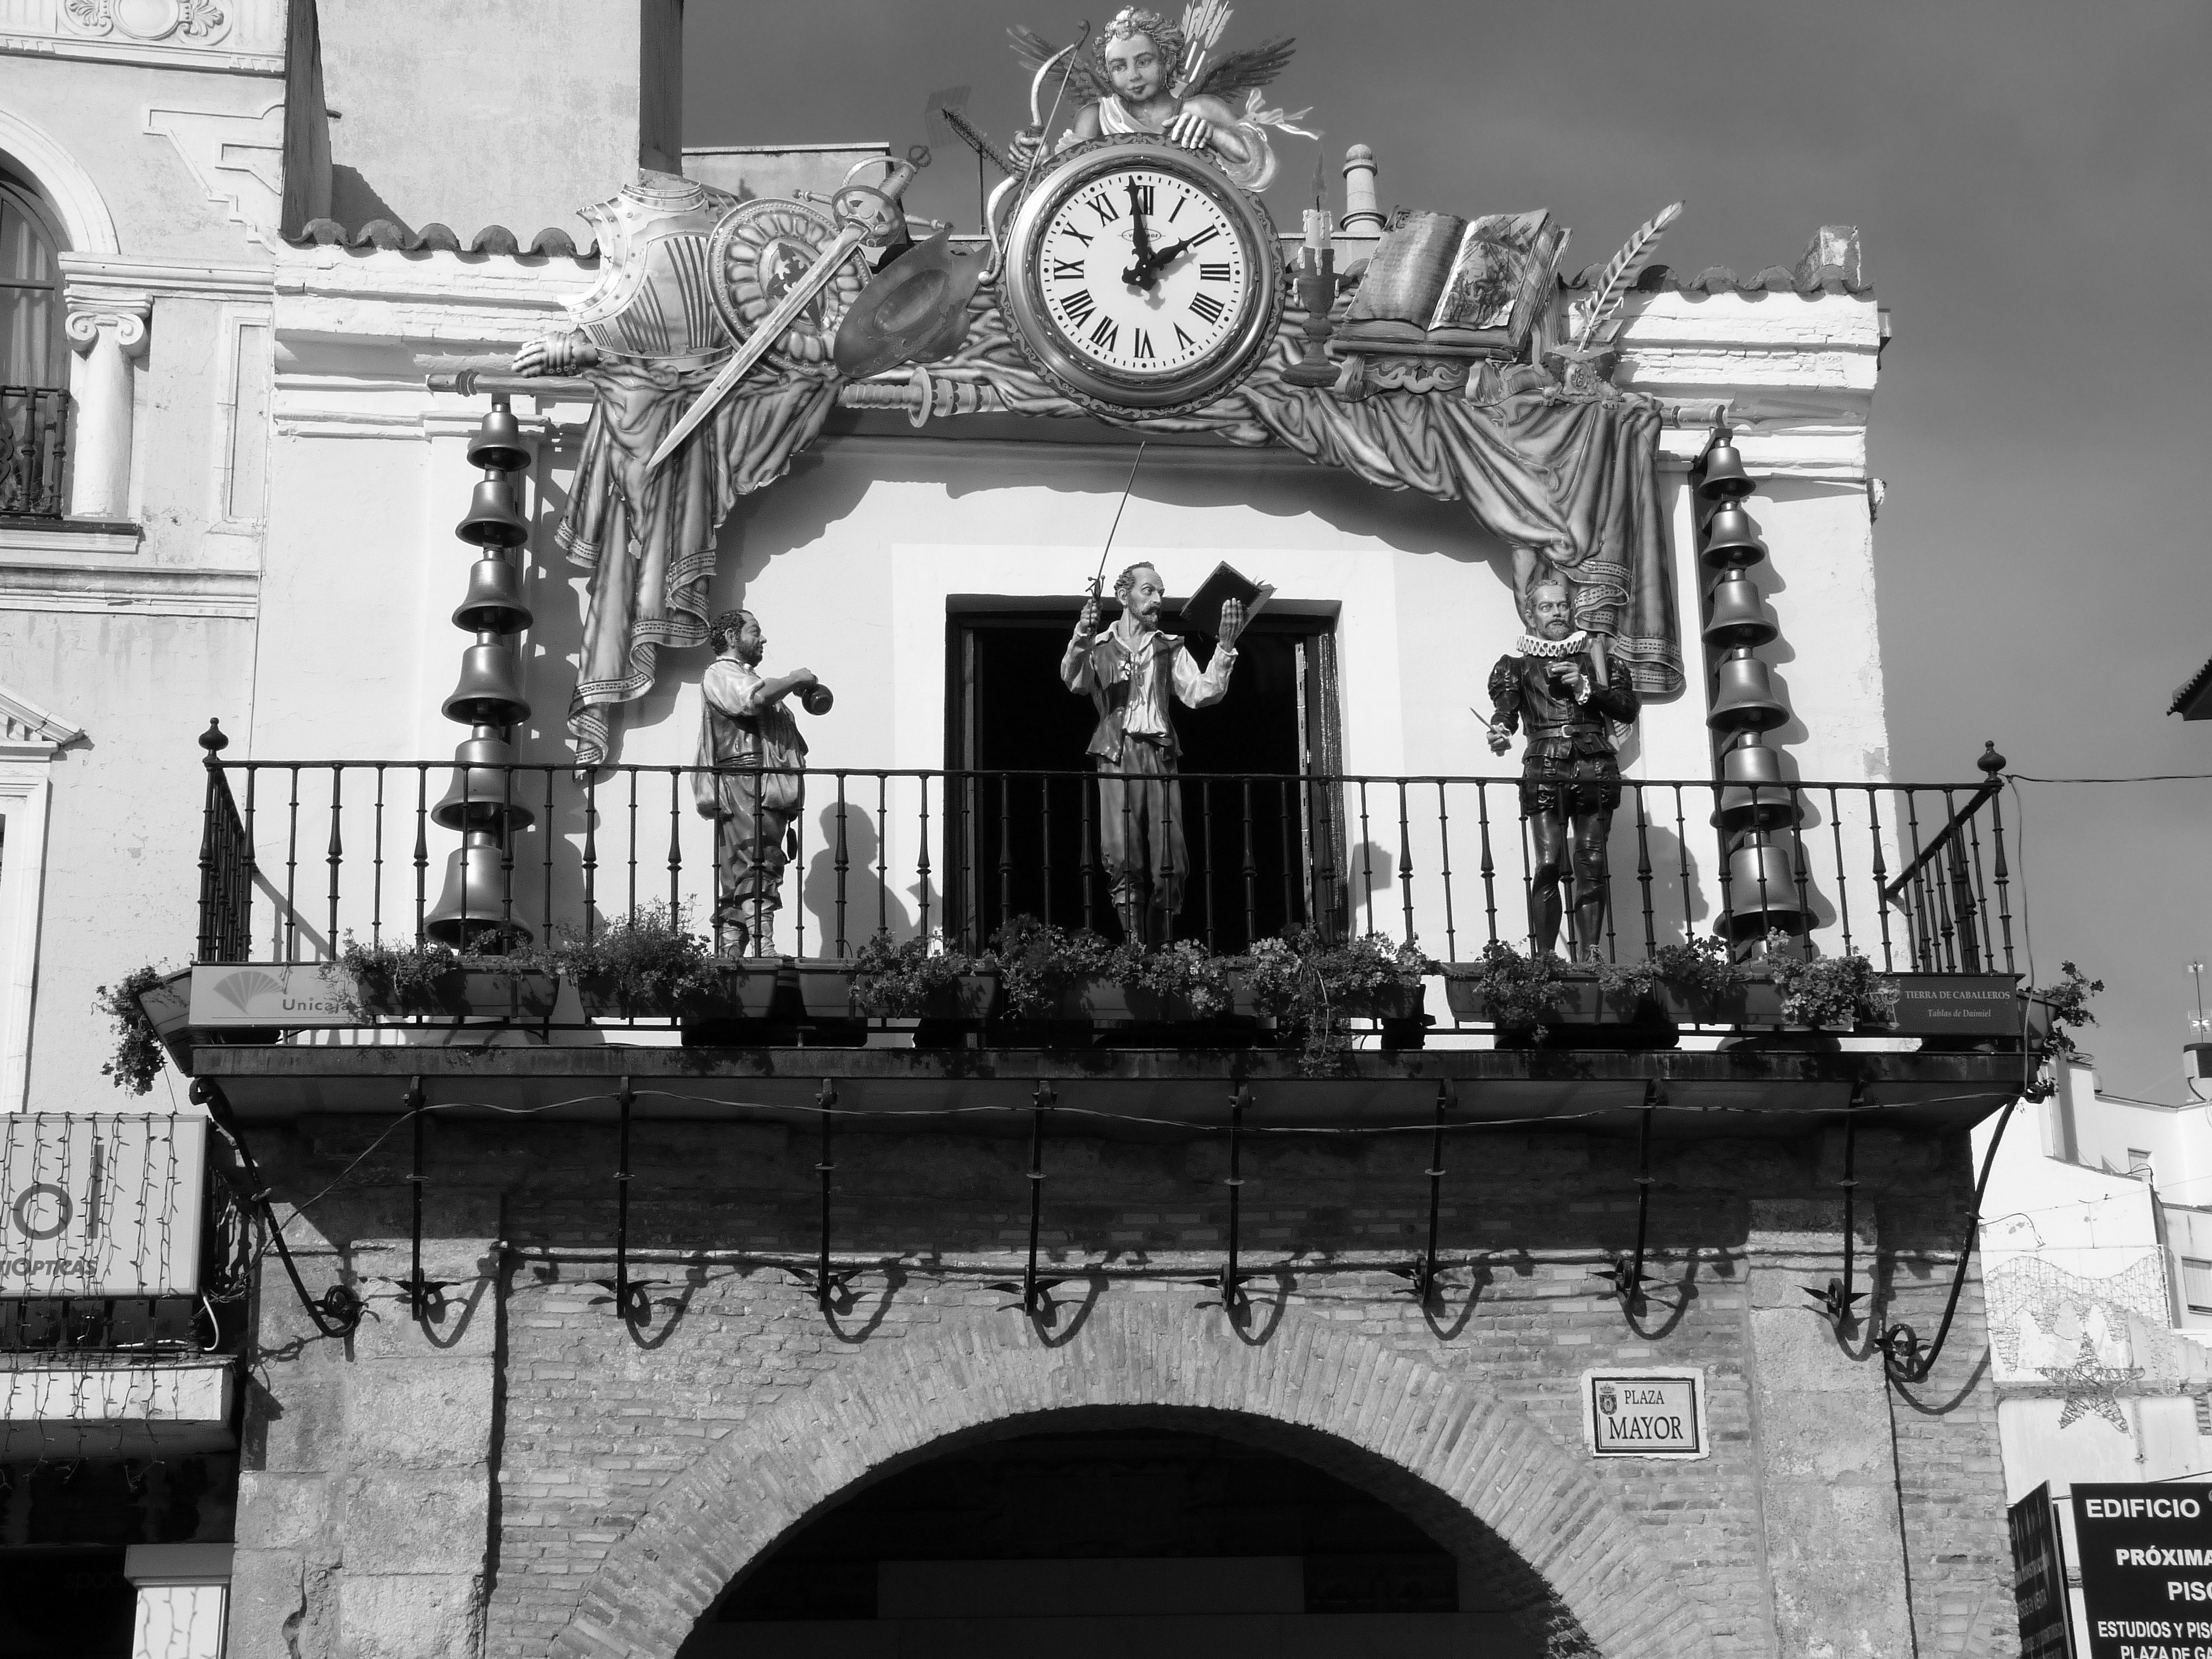
\includegraphics[width=0.8\linewidth]{clockCRbw}
		\caption{Fotografía en blanco y negro}\label{fig:fotoBW}
	\end{subfigure} 
	\caption[Ejemplo de subfiguras]{Ejemplo de inclusión de subfiguras en un mismo entorno (por J. Salido, CC BY-NC-ND)}
	\label{fig:ejSubfigures}
\end{figure}



Mediante el uso de etiquetas (\texttt{\textbackslash label}) es posible incluir referencias cruzadas a subfiguras como la fotografía en blanco y negro de la Fig.~\ref{fig:fotoBW}.

En los trabajos académicos la inclusión de imágenes y figuras que no son propiedad del autor suscitan bastante controversia y son fuente de incumplimiento inadvertido de la ley de propiedad intelectual.\index{plagio!propiedad intelectual} Es importante recordar que \emph{<<el desconocimiento de la ley no exime de su cumplimiento>>} por lo que se recomienda tanto a estudiantes como tutores consultar documentación informativa sobre el uso correcto de figuras en documentos académicos \cite{unican18}. Entre las <<incorrecciones>> más frecuentes al incluir figuras en los documentos académicos se observan:
\begin{itemize}
\item Abuso del derecho de cita. Se produce al incluir, con fines exclusivamente decorativos o ilustrativos de la explicación, una figura sujeta a derechos de uso restringido invocando el derecho de cita (incluso con correcta atribución de la obra).

\item Incorrecta atribución de la obra.\index{atribución} Es habitual confundir al autor de la obra con la fuente de origen de la misma. La fuente es precisa cuando se cita la obra original. Sin embargo, la licencia de muchas obras exige la atribución al autor y la inclusión de la licencia bajo la que se distribuye o hace uso de la misma (véase como ejemplo cómo se realiza una correcta atribución en las Fig.~\ref{fig:ejFigure} y \ref{fig:ejSubfigures} mencionando al autor y la licencia Creative-Commons\footnote{\url{https://creativecommons.org}} bajo la que se rige el uso de la imagen y el mecanismo de título alternativo para que dicha atribución no aparezca en el índice de figuras).\index{Creative Commons}

\item Supresión de denominación de licencia de uso. Al incluir obras de terceros debemos tener presente los términos de distribución de la misma e incluirlos junto a la atribución de su legítimo autor.
\end{itemize}

La inclusión de material de \emph{dominio público}\index{dominio público} o sin restricciones de uso hace innecesaria la atribución al autor pero puede incluirse una nota de agradecimiento.\footnote{Por cortesía de \emph{<x>}.}

\section{Ejemplos de listados}
\label{sec:ejListados}
\index{ejemplos!listados}

Ejemplos más representativos de inclusión de porciones de código 
fuente.\index{listados}

% Ejemplo: Listado Java
% ============
\begin{lstlisting}[language=Java,float=ht,caption={[Código fuente en Java]Ejemplo de código fuente en lenguaje Java},label=lst:java]
// @author www.javadb.com
public class Main {    
// Este método convierte un String a un vector de bytes

public void convertStringToByteArray() {

String stringToConvert = "This String is 15";      
	byte[] theByteArray = stringToConvert.getBytes();        
	System.out.println(theByteArray.length);        
}

public static void main(String[] args) {
	new Main().convertStringToByteArray();
}
}
\end{lstlisting}



\noindent Otro ejemplo.

\begin{lstlisting}[style=C-ruled,float=ht,caption={Ejemplo de código C},label=lst:codC]
// Este código se ha incluido tal cual está en el fichero \LaTeX{}
#include <stdio.h>

int main(int argc, char* argv[]) {
	puts("¡Hola mundo!");
}
\end{lstlisting}


\noindent Ejemplo de entrada por consola.

\begin{lstlisting}[style=consola, numbers=none]
$ gcc -o Hola HolaMundo.c
\end{lstlisting}


\subsection{Algoritmos con el paquete \texttt{algorithm2e}}
Como ya se ha comentado en los textos científicos relacionados con las 
TIC\footnote{Por supuesto en un TFG (Trabajo Fin de Grado)\index{TFG} o tesis 
de un centro superior de informática.} (Tecnologías de la Información y 
Comunicaciones) suelen aparecer porciones de código en los que se explica 
alguna función o característica relevante del trabajo que se expone. Muchas 
veces lo que se quiere ilustrar es un algoritmo o método en que se ha 
resuelto un problema abstrayéndose del lenguaje de programación concreto en 
que se realiza la implementación. El paquete 
\texttt{algorithm2e}\footnote{\url{https://osl.ugr.es/CTAN/macros/latex/contrib/algorithm2e/doc/algorithm2e.pdf}}\index{CTAN}
 proporciona un entorno \texttt{algorithm} para la impresión apropiada de 
algoritmos tratándolos como objetos flotantes y con mucha flexibilidad de 
personalización. En el algoritmo \ref{alg:como} se muestra cómo puede 
emplearse dicho paquete. En este curso no se explican las posibilidades del 
paquete más en profundidad ya que excede el propósito del curso. A todos los 
interesados se les remite a la documentación del mismo.


% Ejemplo:
% ============
\IncMargin{1em}
\begin{algorithm}
\SetKwInOut{Input}{Datos}\SetKwInOut{Output}{Resultado}
\LinesNumbered
\SetAlgoLined

\Input{este texto} 
%\KwIn{este texto}
\Output{como escribir algoritmos con \LaTeX2e}
%\KwOut{como escribir algoritmos con \LaTeX2e}

inicialización\;
\While{no es el fin del documento}{
	leer actual\;
	\eIf{comprendido}{
		ir a la siguiente sección\;
		la sección actual es esta\;
	}{
		ir al principio de la sección actual\;
	}
}

% Aunque el captión aparece abajo siempre se pone arriba como en tablas y listados
\caption{Cómo escribir algoritmos}\label{alg:como}
\end{algorithm}\DecMargin{1em}


\section{Menús, paths y teclas con el paquete \texttt{menukeys}}
Cada vez es más usual que los trabajos en ingeniería exijan el uso de 
software. Para poder especificar de modo elegante el uso menús, pulsación de 
teclas y directorios se recomienda el uso del paquete 
\texttt{menukeys}.\footnote{\url{https://osl.ugr.es/CTAN/macros/latex/contrib/menukeys/menukeys.pdf}}
 \index{CTAN} Este paquete nos permite especificar el acceso a un menú, por 
ejemplo:

\menu{Herramientas > Órdenes > PDFLaTeX}\\

\noindent También un conjunto de teclas. Por ejemplo:
\keys{\ctrl + \shift + T}\\

\noindent O un directorio:
\directory{C:/user/LaTeX/Ejemplos}\\

\noindent Aunque este paquete permite muchas opciones de configuración de los estilos aplicados, no es necesario hacerlo para obtener unos resultados muy elegantes.
